%!TEX root = ../main.tex

\pmax{Think story!}

We describe our novel symbolic execution engine for \jsil, an intermediate
representation for JavaScript analysis previously introduced by \citet{javert}. 
In \S\ref{subsec:jsil:analysis:formalism}, we define an abstract semantics for 
\jsil, which we then instantiate to obtain its concrete and symbolic semantics.
In \S\ref{sex:formal:guarantees}, we present the formal guarantees of 
our symbolic analysis, including: \dtag{i} a soundness result for the \jsil symbolic 
execution, \dtag{ii} a guarantee of absence of false positives for bug-finding, \pmaxinline{Do we know what bug-finding is here?}
\dtag{iii} a justification result for the lifting of analyses on compiled \jsil code back to JavaScript;
and \dtag{iv} \polish{a verification result that precisely states the conditions 
under which symbolic execution gives us verification guarantees.}
Finally, in \S\ref{subsec:jsil:analysis:implementation}, we give a brief overview
of our implementation. %in \rosette~\cite{Rosette1,Rosette2} NO NO NO! Burn the witch!


\subsection{Symbolic Semantics}\label{subsec:jsil:analysis:formalism}

\subsubsection{Syntax} 
\jsil is a simple goto language featuring top-level procedures and commands operating on object heaps. It was purposefully designed to natively support the main dynamic features of JavaScript: extensible objects; dynamic property access; and dynamic procedure calls. The syntax of \jsil is shown below. 

\vspace{5pt}
\begin{display}{Syntax of the \jsil Language}{
\begin{tabular}{llllll}
	 Numbers: $\jnumber \in \numbers$ &  Booleans: $\jbool \in \bools$ & \  \ Strings: $\jstring \in \strings$ & \  \ Locations: $\loc \in \locs$ & \  Vars: $\jvar \in \jvars$ & \ Types: $\jtype \in \jtypes$ \\[0.1cm]
\multicolumn{6}{l}{Values: $\val \in \vals$ \defeq \ $\jnumber \! \mid \! \jbool \! \mid \! \jstring \! \mid \! \jundefined \! \mid \! \jnull \! \mid \! \jempty \! \mid \! \loc \! \mid \! \jtype \! \mid \!  \pid$ \qquad Expressions: $\jsilexpr \in \exprs$ \defeq \ $\val \mid \jvar \mid \ominus\ \jsilexpr \mid \jsilexpr \binop{} \jsilexpr $} \\[0.1cm]
	\multicolumn{6}{l}{Basic Commands: $\bcmd \in \bcmds$ \defeq\ $\jsilskip \mid \jvar := \jsilexpr  \mid \jvar := \jsilnew() \mid \jvar := [\jsilexpr, \jsilexpr] \mid [\jsilexpr, \jsilexpr] := \jsilexpr \mid$} \\[0.1cm]
	\multicolumn{6}{l}{\hspace{3.29cm} $\jsildelete(\jsilexpr, \jsilexpr) \mid \jvar := \hasfield(\jsilexpr, \jsilexpr) \mid \jvar := \getfields(\jsilexpr) \mid \jvar := \makesymbolic(\jtype)$} \\[0.1cm]
	% Commands
	\multicolumn{6}{l}{Commands: $\jcmd \in \cmds$ \defeq \ $ \bcmd \mid \goto \ i \mid  \ifgoto{\jsilexpr}{i}{j} \mid \jsilcall{\jvar}{\jsilexpr}{\jvec{\jsilexpr}}{j} 
	         \mid \assume(\jsilexpr) \mid \assert(\jsilexpr)$} \\[0.1cm]
	\multicolumn{6}{l}{Procedures : $\proc \in \procs$ \defeq \ $\procedure{\pid}{\jvec{\jvar}}{\jvec{\jcmd}}$}
 \end{tabular}}
\end{display}

\vspace{5pt}
\noindent \jsil \emph{values}, $\val \in \vals$, include numbers, booleans, strings, the special values $\jundefined$, $\jnull$, and $\jempty$, as well as types~$\jtype$, and procedure identifiers $\pid$.
\jsil~\emph{expressions}, $\jsilexpr \in \exprs$, include \jsil values, \jsil program variables $\jvar$, and various unary and binary operators, which, for instance, provide support for sets and lists. 

\jsil \emph{basic commands} enable the manipulation of extensible objects and do not affect control flow. 
They include $\jsilskip$, variable assignment, object creation, property access, property assignment, property deletion, membership check,  property collection, and symbolic variable creation. 

\jsil \emph{commands} include \jsil basic commands and commands related to control flow: conditional and unconditional gotos, dynamic procedure calls, and two special commands, $\assume$ and $\assert$, essential for symbolic execution, but with trivial concrete semantics.\footnote{\jsil also has a $\phi$-node assignment, which allows \JSComp to produce code directly in Static-Single-Assignment (SSA) \cite{SSA}. To avoid clutter, we omit the $\phi$-node assignment from the formal presentation as it does not impact the reasoning. Details can be found in \cite{javert}.} 
The two goto commands are straightforward: $\goto \ i$ jumps to the $i$-th command of the active procedure, and $\ifgoto{\jsilexpr}{i}{j}$ jumps to the $i$-th command if $\jsilexpr$ evaluates to $\jtrue$, and to the $j$-th if it evaluates to $\jfalse$. 
The dynamic procedure call $\jsilcall{\jvar}{\jsilexpr}{\jvec{\jsilexpr}}{j}$ first evaluates  $\jsilexpr$ and $\jvec{\jsilexpr}$ to obtain the procedure identifier and arguments, respectively, executes the appropriate procedure with these arguments, and, in the end, assigns its return value to $\jvar$.
If the procedure raises an error, control is transferred to the $j$-th command; otherwise, it simply follows to the next command. 

A \jsil program $\prog \in \progs$ can be seen as a set of top-level procedures of the form $\procedure{\pid}{\jvec{\jvar}}{\jvec{\jcmd}}$, where $\pid$ is the procedure identifier, $\jvec{\jvar}$ are its formal parameters, and its body ${\jvec{\jcmd}}$  is a sequence of \jsil commands.
Every \jsil program contains a special procedure $\jsilmain$\hspace{-2pt}, denoting the entry point of the program. 
\jsil procedures return via two dedicated indexes, $\retlab$ and $\errlab$, using two dedicated variables, $\retvar$ and $\errvar$. If a procedure reaches the $\retlab$ index, it returns normally with the return value denoted by $\retvar$; when it reaches $\errlab$, it returns an error, with the error value denoted by $\errvar$.

%

\subsubsection{Abstract Semantics}
We first define an abstract semantics for \jsil, which is parametric on a \jsil \emph{state signature}. 
Then, we instantiate this abstract semantics with a concrete state signature to obtain the \emph{concrete semantics} for \jsil, and with a symbolic state signature to obtain its symbolic counterpart.
This approach to the design of symbolic analyses has the following main benefits: \dtag{1} it streamlines the formalism, avoiding redundancy,
\dtag{2} it makes explicit the choices in the design of the symbolic semantics,
and \dtag{3} it leads to modular implementations, avoiding code duplication.


The abstract semantics is parametric on abstract states $\absstate \in \absstates$ and abstract values $\absval \in \absvals$.
Abstract states are assumed to have a store component $\absstore: \jvars \partialmap \absvals$, mapping program variables $\jvar \in \jvars$ to abstract values. Abstract values must include: \jsil values, $\val$; abstract locations, $\absloc$; abstract property names, $\absprop$; sets of abstract values; and the special value $\none$, used to indicate the absence of a property in an object. Abstract states expose the following functions and relations: 
\begin{description}
\setlength{\itemsep}{0.2em}
  \item[\jsil Expression Evaluation,] $\evalexpr{} :  (\jvars \partialmap \absvals)  \partialmap \exprs \partialmap \absvals$. 
  	The expression $\evalexpr{}(\absstore, \jsilexpr)$ evaluates to the abstract value of the \jsil expression $\jsilexpr$ under store $\absstore$. 
            
  \item[Store Selector,] $\stosel : \absstates \rightarrow (\jvars \partialmap \absvals)$. The expression $\stosel(\absstate)$ evaluates to the abstract store associated with a given abstract state $\absstate$. For clarity, we write $\absstate.\stosel$ instead of $\stosel(\absstate)$. 
             
  \item[Store Update,] $\stupdt{}: \absstates \rightarrow \jvars \rightarrow \absvals \rightarrow \absstates$. 
             The expression $\stupdt{}(\absstate, \jvar, \absval)$ denotes the abstract state obtained from $\absstate$ 
             by updating the abstract value corresponding to $\jvar$ in $\absstate.\stosel$ to $\absval$. 

   \item[Heap Update,] $\hpupdt{} : \absstates \rightarrow \absvals \partialmap \absvals \partialmap \absvals \partialmap \absstates$. 
             The expression $\hpupdt{}(\absstate, \absloc, \absprop, \absval)$ denotes the abstract state obtained from $\absstate$ 
             by updating the value of property $\absprop$ of the object at location $\absloc$ to $\absval$. 
                   
  
  \item[GetCell,] $\getcell \subseteq \absstates \times \exprs \times \exprs \times \absstates \times \absvals \times \absvals \times \absvals$. 
          We pretty-print $(\absstate, \jsilexpr_1, \jsilexpr_2, \absstate', \absloc, \absprop, \absval) \in \getcell$ as $\absgetcellrule{}{\absstate, \jsilexpr_1, \jsilexpr_2}{\absstate', (\absloc, \absprop, \absval)}$. 
          Informally, GetCell retrieves the value associated with a given property of a given object. More formally, if $\absgetcellrule{}{\absstate, \jsilexpr_1, \jsilexpr_2}{\absstate', (\absloc, \absprop, \absval)}$ holds, 
          then \dtag{1} $\absloc$ denotes the abstract location resulting from the evaluation of $\jsilexpr_1$, 
          \dtag{2} $\absprop$ denotes the abstract property name resulting from the evaluation of $\jsilexpr_2$, 
          \dtag{3} $\absval$ denotes the abstract value of the property $\absprop$ of the object at location $\absloc$, 
          and \dtag{4} $\absstate'$ denotes a (potential) modification of $\absstate$ that allows for the property inspection (discussed shortly). 
          Note that $\getcell$ is non-deterministic and is, therefore, a relation.
             
  \item[GetDomain,] $\getdomain \subseteq \absstates \rightarrow \exprs \partialmap \absvals$. 
           We pretty-print $(\absstate, \jsilexpr, \absval) \in \getdomain$ as $\absgetdomainrule{}{\absstate, \jsilexpr}{\absval}$. 
           If $\absgetdomainrule{}{\absstate, \jsilexpr}{\absval}$ holds, then $\absval$ denotes the 
           set of abstract property names associated with the object at the location resulting from the evaluation of $\jsilexpr$ 
           in $\absstate$. 
   
   \item[Assumption,] $\absassume{} : \absstates \rightarrow \exprs \partialmap \absvals$. 
            The expression $\absassume{}(\absstate, \jsilexpr)$ denotes the abstract state obtained from the 
            abstract state $\absstate$ by assuming that $\jsilexpr$ evaluates to the boolean $\jtrue$. 
  
   \item[Satisfiability,] $\abssat{} : \absstates \rightarrow \exprs \partialmap \bools$. 
            The expression $\abssat{}(\absstate, \jsilexpr)$ evaluates to $\jtrue$ if the \jsil expression $\jsilexpr$ is \polish{satisfiable} in the abstract 
            state $\absstate$, and $\jfalse$ otherwise.
             
   \item[Symbolic Value Creation,] $\absmakesymbolic : \jtypes \rightarrow \absvals$. 
            The expression $\absmakesymbolicrule{}{\jtype}$ evaluates to a fresh symbolic value of type $\jtype$.
\end{description}

\begin{figure}[ht!]
{\scriptsize
\begin{mathpar}
  \inferrule[\textsc{Skip}]{}
	{ \absbsemrule{\absstate, \jsilskip}{\absstate}{}}  	
\and 
\inferrule[\textsc{Property Collection}]
  {
           \absgetdomainrule{}{\absstate, \jsilexpr}{\absval}  
  }{\absbsemrule{\absstate, \jvar := \getfields(\jsilexpr)}{\stupdt{}(\absstate, \jvar, \absval)}{}} 
\and 
\inferrule[\textsc{Assignment}]
  {
        \absstore = \absstate.\stosel
        \quad 
        \absval = \evalexpr{}(\absstore, \jsilexpr)
  }{\absbsemrule{\absstate, \jvar := \jsilexpr}{\stupdt{}(\absstate, \jvar, \absval)}{}} 
\\
\inferrule[\textsc{Object Creation}]
  { 
   \loc \text{ fresh}
  }{\absbsemrule{\absstate, \jvar := \jsilnew()}{\hpupdt{}(\absstate, \loc, \protop, \jnull)}{}}
\and 
\inferrule[\textsc{Property Access}]
  { 
  	\absgetcellrule{}{\absstate, \jsilexpr_1, \jsilexpr_2}{\absstate', (-, -, \absval)}
  }{ \absbsemrule{\absstate, \jvar := [\jsilexpr_1, \jsilexpr_2]}{\stupdt{}(\absstate', \jvar, \absval)}{}}
%
\\
\inferrule[\textsc{Property Assignment}]
  {    
      \absgetcellrule{}{\absstate, \jsilexpr_1, \jsilexpr_2}{\absstate', (\absloc, \absprop, -)} \quad \absstore = \absstate.\stosel \quad \absval = \evalexpr{}(\absstore, \jsilexpr_3)
  }{\absbsemrule{\absstate, [\jsilexpr_1, \jsilexpr_2] := \jsilexpr_3}{\hpupdt{}(\absstate', \absloc, \absprop, \absval)}{}} 
\and
 \inferrule[\textsc{Property Deletion}]
  { 
        \absgetcellrule{}{\absstate, \jsilexpr_1, \jsilexpr_2}{\absstate', (\absloc, \absprop, \absval)}
        \quad
     	\absval \neq \none
  }{\absbsemrule{\absstate, \jsildelete(\jsilexpr_1, \jsilexpr_2)}{\hpupdt{}(\absstate', \absloc, \absprop, \none)}{}}
\\
\inferrule[\textsc{Member Check - True}]
  { 
     \absgetcellrule{}{\absstate, \jsilexpr_1, \jsilexpr_2}{\absstate', (-, -, \absval)} 
     \quad 
    \absval \neq \none
  }{\absbsemrule{\absstate, \jvar := \hasfield(\jsilexpr_1, \jsilexpr_2)}{	{}(\absstate', \jvar, \jtrue)}{}}
 \and 
\inferrule[\textsc{Member Check - False}]
  { 
     \absgetcellrule{}{\absstate, \jsilexpr_1, \jsilexpr_2}{\absstate', (-, -, \none)} 
  }{\absbsemrule{\absstate, \jvar := \hasfield(\jsilexpr_1, \jsilexpr_2)}{\stupdt{}(\absstate', \jvar, \jfalse)}{}} \\
  \inferrule[\textsc{Make Symbolic}]
  { 
     \absval = \absmakesymbolicrule{}{\jtype}
  }{\absbsemrule{\absstate, \jvar := \makesymbolic(\jtype)}{\stupdt{}(\absstate, \jvar, \absval)}{}}
\end{mathpar}}
 \vspace*{-0.6cm}
\caption{Abstract Semantics for Basic Commands: {\scriptsize$\absbsemrule{\absstate, \bcmd}{\absstate'}{}$}\label{abs:sem:bcmds:fig}}
\end{figure}

\begin{figure}[ht!]
{\scriptsize
\begin{mathpar} 
\inferrule[\textsc{Basic Command}]
   { 
     \ccmd[\prog][\abscs]{i} = \bcmd 
     \\\\
     \absbsemrule{\absstate, \bcmd}{\absstate'}{} 
   }{\abssemrule{\absstate, \abscs, i}{\absstate', \abscs, i{+}1}{\top}{\top}{}}
  %
  \and
  %
  \inferrule[\textsc{Cond. Goto - True}]
   { \ccmd[\prog][\abscs]{i} =  \ifgoto{\jsilexpr}{j}{k} 
     \\\\
     %   \absval = \evalexpr{}(\absstate.\stosel, \jsilexpr)
     %   \quad 
     \absstate' = \absassume{}(\absstate, \jsilexpr) 
   }
   {\abssemrule{\absstate, \abscs, i}{\absstate', \abscs, j}{\top}{\top}{}}
  %
  \and 
  % 
  \inferrule[\textsc{Cond. Goto - False}]
   { \ccmd[\prog][\abscs]{i} =  \ifgoto{\jsilexpr}{j}{k} 
      \\\\ 
       % \absval = \evalexpr{}(\absstate.\stosel, \jsilexpr)
       % \quad 
      \absstate' = \absassume{}(\absstate, \neg\jsilexpr) 
   }
   {\abssemrule{\absstate, \abscs, i}{\absstate', \abscs, k}{\top}{\top}{}}
  %
  \\
  %
  \inferrule[\textsc{Goto}]
   { 
   \ccmd[\prog][\abscs]{i} = \goto \, j \quad}
   {\abssemrule{\absstate, \abscs, i}{\absstate, \abscs, j}{\top}{\top}{}}
   %
   \qquad 
   %
   \inferrule[\textsc{Normal Return}]
   {
       \abscs = (-, \absstore', \jvar, i, -) :: \abscs'  
       \quad 
       \absstore = \absstate.\stosel
       \\\\
       \absstate' = \absstate[\stosel \mapsto \absstore'[\jvar \mapsto \absstore(\retvar)]]
   }  
   {\abssemrule{\absstate, \abscs, \retlab}{\absstate', \abscs', i}{\top}{\top}{}}
     %
   \qquad 
   %
      \inferrule[\textsc{Error Return}]
   { 
       \abscs = (-, \absstore', \jvar, -, j) :: \abscs'
       \quad 
       \absstore = \absstate.\stosel
       \\\\
       \absstate' = \absstate[\stosel \mapsto \absstore'[\jvar \mapsto \absstore(\errvar)]]
   }  
   {\abssemrule{\absstate, \abscs, \errlab}{\absstate', \abscs', j}{\top}{\top}{}}
      \\
    \inferrule[\textsc{Procedure Call}]
   { 
    \ccmd[\prog][\abscs]{i} =   \jsilcall{\jvar}{\jsilexpr}{\jsilexpr_i \mid_{i = 0}^{n}}{j}
     \and
     \absstore = \absstate.\stosel 
     \and 
    \evalexpr{}(\absstore, \jsilexpr) =  \pid' 
        \and
     \args(\prog, \pid') = \jsillist{\jvar_1, ..., \jvar_{m}} 
      \\\\
      \absval_i = \evalexpr{}(\absstore, \jsilexpr_i) \mid_{i = 0}^{n} 
     \and
      \absval_i = \jundefined \mid_{i = n+1}^{m}  
      \and 
      \absstore' = [ \jvar_i \mapsto \absval_i \mid_{i = 0}^{m}]
      \and 
      \abscs' = (\pid', \absstore, \jvar, i{+}1, j) :: \abscs 
   }
   {\abssemrule{\absstate, \abscs, i}{\absstate[\stosel \mapsto \absstore'], \abscs', 0}{\top}{\top}{}}
    \\ 
%
\inferrule[\textsc{Assume}]
  { 
      \ccmd[\prog][\abscs]{i}  = \assume(\jsilexpr) 
      \\\\ 
      %\absstore = \absstate.\stosel
      %\quad
      %\evalexpr{}(\absstore, \jsilexpr) =  \absval
      %\\\\
     \absstate' = \absassume{}(\absstate, \jsilexpr) 
  }{\abssemrule{\absstate, \abscs, i}{\absstate', \abscs, i{+}1}{\top}{\top}{}} 
\and
\inferrule[\textsc{Assert - True}]
  { 
      \ccmd[\prog][\abscs]{i}  = \assert(\jsilexpr)
      \\\\ 
      %\absstore = \absstate.\stosel
      %\quad
      %\absval = \evalexpr{}(\absstore, \jsilexpr)
      % \\\\
       \abssat(\absstate, \neg \jsilexpr) = \jfalse
  }{\abssemrule{\absstate, \abscs, i}{\absstate, \abscs, i{+}1}{\top}{\top}{}} 
\and 
\inferrule[\textsc{Assert - False}]
  { 
      \ccmd[\prog][\abscs]{i}  = \assert(\jsilexpr)
      \\\\ 
      %\absstore = \absstate.\stosel
      %\quad
      %  \absval = \evalexpr{}(\absstore, \jsilexpr)
      % \\\\
      \abssat(\absstate, \neg \jsilexpr) = \jtrue
  }{\abssemrule{\absstate, \abscs, i}{\absstate, \abscs, i}{\top}{\bot}{}} 
 \end{mathpar}}
% \pmax{What happens when we exit from main, how do we stop? Basically, cmd returns nothing and we can't reduce?}
 \vspace*{-0.6cm}
\caption{Abstract Execution for Control Flow Commands: $\abssemrule{\absstate, \abscs, i}{\absstate', \abscs', j}{\mode}{\mode'}{}$}
\label{abs:sem:cmds:fig}
\end{figure}

Transitions for basic commands and control flow commands are given 
in Figures~\ref{abs:sem:bcmds:fig} and~\ref{abs:sem:cmds:fig}. Transitions for 
basic commands are of the form 
$\absbsemrule{\absstate, \bcmd}{\absstate'}{}$, meaning that the execution of the basic command 
$\bcmd$ in the abstract state $\absstate$ results in the abstract state $\absstate'$. 
%
To describe transitions for control flow commands, we introduce \emph{execution modes} and 
\emph{call stacks}.  \jsil has two execution modes, ranged over by $\mode$: 
$\top$, which indicates that the execution can proceed; and~$\bot$, which indicates that a failure 
has occurred and the execution must stop. Call stacks, ranged over by $\abscs$, are lists of tuples of the form $(\pid, \absstore, \jvar, i, j)$, where: 
\dtag{1}~$\pid$~is the identifier of the procedure that is currently executing;
\dtag{2}~$\absstore$~is the store of the procedure that called $\pid$; 
\dtag{3}~$\jvar$~is the variable to which the return of $\pid$ must be assigned in $\absstore$; 
\dtag{4} $i$ is the index of the command to which the control must jump after the execution of $\pid$ in case of normal return; 
and \dtag{5} $j$ is the index to which it must jump in case of error return. 
Transitions for control flow commands have the form:  $\abssemrule{\absstate, \abscs, i}{\absstate', \abscs', j}{\mode}{\mode'}{}$, 
meaning that, in the context of the entire program $\prog$, the evaluation of the $i$-th command of the first procedure in the 
call stack $\abscs$, in state $\absstate$ and execution mode $\mode$, generates 
the state $\absstate'$, call stack $\abscs$,  and the next command to be evaluated is the $j$-th command of the first procedure 
of the call stack~$\abscs'$, in execution mode $\mode'$. 
For clarity, we keep the executing program implicit and make use of a function $\ccmd{\prog, \cs, i}$, which 
returns the $i$-th command of the procedure that is first in $\cs$. %We write $\ccmd{i}$ when $\prog$ and $\ctx$ are implicit.

\jfs{
\begin{enumerate}
   \item Should we explain the rules?
   \item We shou
\end{enumerate}
}

\subsubsection{Concrete Semantics}
A \jsil concrete state $\jstate$ is a pair $(\heap, \store)$ consisting of a heap and a store. 
A heap, $\heap \in \heaps$, is a partial function mapping pairs of  object locations and property names (strings) to \polish{\jsil values},
whereas a store, $\store \in \stores$, maps \jsil program variables to \jsil values. 
Given a heap~$\heap$, we denote: the empty heap by $\hemp$; heap lookup by $\heap(\loc, \jstring)$; 
a heap cell by $\hcell{\loc}{\jstring}{\val}$, meaning that  $\heap(\loc,\jstring) = \val$; 
heap update by $\heap[(\loc, p) \mapsto \val]$, denoting the heap $\heap$ extended with $\heap(\loc,\jstring) = \val$;
and the union of two disjoint heaps by $\heap_1 \dunion \heap_2$.
We instantiate the abstract semantics for the concrete case by providing the appropriate definitions 
for the required abstract functions/relations below, noting that abstract values are instantiated to
\jsil values extended with the property absence indicator $\none$.
We write $\absbsemrule{\jstate, \bcmd}{\jstate'}{\concrete}$ for the concrete semantic 
judgement for basic commands and $\abssemrule{\jstate, \cs, i}{\jstate', \cs', j}{\mode}{\mode'}{\concrete}$ 
for control flow commands. 

\begin{display}{Concrete Semantics Rules}
\text{
{\scriptsize
\begin{mathpar} 
  \inferrule[\textsc{Expression Evaluation}]
  {}{\evalexpr{\concrete}(\store, \val) = \val \qquad 
  	\evalexpr{\concrete}(\store, \jvar) = \store(\jvar) \qquad 
	\evalexpr{\concrete}(\store, \ominus \jsilexpr) = \semop{\ominus} \ \evalexpr{c}(\store, \jsilexpr) \qquad
	\evalexpr{\concrete}(\store, \jsilexpr_1 \oplus \jsilexpr_2) = \evalexpr{c}(\store, \jsilexpr_1) \ \semop{\oplus} \ \evalexpr{c}(\store, \jsilexpr_2)}
  \\
  \inferrule[\textsc{GetDomain}]
   { 
        \evalexpr{c}(\store, \jsilexpr) = \loc
      \quad
       \heap = \heap' \, \uplus \, \big((\loc, p_i) \mapsto \val_i \big)\mid_{i = 0}^m  
      \quad
          (\loc,-) \notin \domain (\heap')  
       }{  \absgetdomainrule{\concrete}{(\heap, \store), \jsilexpr}{\jsilset{p_1, ..., p_m}}}
  %
  \and
  %
    \inferrule[\textsc{GetCell - Explicit Cell}]
   { 
         \evalexpr{c}(\store, \jsilexpr_1) = \loc
        \quad 
         \evalexpr{}(\store, \jsilexpr_2) = p
        \quad
       \heap = - \, \uplus \, (\loc, p) \mapsto \val
        }{  \absgetcellrule{\concrete}{(\heap, \store), \jsilexpr_1, \jsilexpr_2}{(\heap, \store), (\loc, p, \val)}}
 %
 \\
   \inferrule[\textsc{Store Selector}]
   {}{  \stosel((\heap, \store)) =  \store}
  	\qquad
   \inferrule[\textsc{Store Update}]
   { 
         \store' = \store[\jvar \mapsto \val]
   }{  \stupdt{\concrete}((\heap, \store), \jvar, \val) =  (\heap, \store')}
   \qquad
       \inferrule[\textsc{Heap Update - Non-$\none$}]
   { 
         \heap' = \heap[(\loc, p) \mapsto \val]
         \quad 
         \val \neq \none
   }{  \hpupdt{\concrete}((\heap, \store), \loc, p, \val) =  (\heap', \store)}
 \qquad
       \inferrule[\textsc{Heap Update - $\none$}]
   { 
         \heap = \heap' \dunion (\loc, p) \mapsto -
   }{  \hpupdt{\concrete}((\heap, \store), \loc, p, \none) =  (\heap', \store)}
  %

   \\
      \inferrule[\textsc{Assumption}]
   {}{  \absassume{\concrete}(\jstate, \jtrue) =  (\jstate, \jtrue) }
\and 
    \inferrule[\textsc{Satisfiability}]
   {}{  \abssat{\concrete}(\jstate, \jbool) = \jbool}
  \and
      \inferrule[\textsc{Symbolic Value Creation }]
   {\val \in \vals \text{ is of type } \jtype}{\absmakesymbolicrule{\concrete}{\jtype} = \val}
 \end{mathpar}
  }}
 \end{display}
  
\pmax{Perhaps a comment on the semantics - eval of expressions and something?}

\subsubsection{Symbolic Semantics}
In order to symbolically execute \jsil programs, we extend the syntax of \jsil expressions with 
symbolic strings $\sstring \in \sstrings$ and symbolic numbers $\snumber \in \snumbers$. 
For convenience, we use $\svars$ to denote the union of $\sstrings$ and $\snumbers$ 
and $\svar$ to range over $\svars$. We introduce: \jsil symbolic expressions, $\sexpr \in \sexprs$, defined as follows: $\sexpr \triangleq \val \mid \svar \mid \unoper\ \sexpr \mid \sexpr \binoper \sexpr$. 
Furthermore, we redefine \jsil expressions, $\pvsexpr \in \pvsexprs$ to take into account symbolic values
 as follows: $\pvsexpr \triangleq \val \mid \jvar \mid \svar \mid \unoper\ \pvsexpr \mid \pvsexpr \binoper \pvsexpr$.
Extended \jsil expressions differ from symbolic expressions in that they can contain program variables.
We extend heaps, stores, and call stacks with symbolic expressions, obtaining symbolic 
heaps, stores, and call stacks, respectively ranged over by $\sheap$, $\sstore$, and $\scs$.
A symbolic heap, $\sheap \in \sheaps$, is a partial function mapping pairs of  
object locations and symbolic expressions to symbolic expressions. 
A symbolic store, $\sstore \in \sstores$, is a mapping from program variables 
$\jvar \in \jvars$ to symbolic expressions. Therefore, an evaluation of a \jsil extended expression $\pvsexpr$ in a symbolic store $\sstore$ always yields a 
symbolic expression $\sexpr$.
A symbolic call stack $\scs$ only differs from a concrete call stack in that it contains 
symbolic stores instead of concrete stores.


A \emph{symbolic state} $\sstate = (\sheap, \sdom, \sstore, \pc)$ is a 4-tuple consisting of a 
symbolic heap $\sheap$, a symbolic domain $\sdom$, a symbolic store $\sstore$, and a path condition $\pc$. 
The \emph{heap domain} maps object locations to set of properties that may be defined in the corresponding object.  
The \emph{path condition}~\cite{symb:exec:survey} is a first-order quantifier-free formula over symbolic strings and 
numbers, which accumulates constraints on the given symbolic inputs that trigger 
the execution to follow the path that led to the current symbolic state.
To avoid clutter, we conflate logical values with \jsil logical values and \jsil logical 
operators with the boolean logical operators. Alternatively, we could have chosen to 
have two different types, \jsil logical expressions and logical expressions, together with a lifting 
function for converting the former to the latter. Our choice simplifies both reasoning 
and~presentation, in that a path condition is simply a \jsil symbolic expression of type boolean. 

We instantiate the abstract semantics for the symbolic case by providing the appropriate definitions 
for the required abstract functions/relations. 
We write $\absbsemrule{\jstate, \bcmd}{\jstate'}{\symbolic}$ for the symbolic semantic 
judgement for basic commands and $\abssemrule{\jstate, \cs, i}{\jstate', \cs', j}{\mode}{\mode'}{\symbolic}$ 
for control flow commands. 

\vspace{5pt}
\begin{display}{Symbolic Semantics Rules}
\text{
{\scriptsize
\begin{mathpar} 
 \inferrule[\textsc{Expression Evaluation}]
  {}{
        {\begin{array}{c}
           \evalexpr{\symbolic}(\sstore, \val) = \val  \\[2pt]
  	   \evalexpr{\symbolic}(\sstore, \jvar) = \sstore(\jvar)  
        \end{array}} \quad
	%
	\frac{
		\sexprv =  \evalexpr{\symbolic}(\sstore, \jsilexpr) \quad
		\sexprv' = \left\{ {\begin{array}{l}
		      \semop{\ominus} (\sexprv) \ \text{if } \sexprv \in \vals \\
		      \ominus \sexprv                   \ \ \ \text{  otherwise}
		 \end{array}} \right. 
	  }{
	    \evalexpr{\symbolic}(\sstore, \ominus \jsilexpr) = \sexprv'
	  } \qquad
	  %
	  \frac{
	     \begin{array}{c}
	         \sexprv_1 = \evalexpr{\symbolic}(\sstore, \jsilexpr_1) \\[2pt]
	         \sexprv_2 = \evalexpr{\symbolic}(\sstore, \jsilexpr_2)  
	     \end{array}    
	     \quad 
	     \sexprv' = \left\{ {\begin{array}{l}
		      \semop{\oplus} (\sexprv_1, \sexprv_2) \ \text{if } \sexprv_1, \sexprv_2 \in \vals \\
		      \sexprv_1 \oplus \sexprv_2      \  \ \ \text{  otherwise}
		 \end{array}} \right. 
	  }{\evalexpr{\symbolic}(\sstore, \jsilexpr_1 \oplus \jsilexpr_2) = \sexprv'}}
\\
  \inferrule[\textsc{GetDomain}]
   { 
        \evalexpr{}(\sstore, \jsilexpr) = \sloc
      \quad
       \sheap = \sheap' \, \uplus \, \big((\sloc, \sexprp_i) \mapsto \sexprv_i \big)\mid_{i = 0}^m  
        \\\\
        %
          (\sloc,-) \notin \domain (\sheap')  
        \quad
         \pc \vdash \jsilset{\sexprp_1, ..., \sexprp_m} = \sdom(\sloc)
         \\\\
        \forall_{0 \leq i \leq n} \, \sexprv_i \neq \none 
         \quad 
           \forall_{n < i \leq m} \, \sexprv_i = \none 
   }{  \absgetdomainrule{\symbolic}{(\sheap, \sdom, \sstore, \pc), \jsilexpr}{\jsilset{\sexprp_1, ..., \sexprp_n}}}
  \and
 % 
     \inferrule[\textsc{GetCell - Not Found}]
   { 
         \evalexpr{}(\sstore, \jsilexpr_1) = \sloc
        \quad 
        \evalexpr{}(\sstore, \jsilexpr_2) = \sexprp
      \quad
       \sheap = \sheap'' \, \uplus \, \big((\sloc, \sexprp_i) \mapsto \sexprv_i \big)\mid_{i = 0}^m
      \\\\
       (\sloc,-) \notin \domain (\sheap'')
        \quad
        \sdom(\sloc) = \sexprv_d
        \quad 
        \sheap' = \sheap[(\sloc, \sexprp) \mapsto \none]
       \\\\ 
       \sdom' = \sdom[\sloc \mapsto \sexprv_d \cup \jsilset{\sexprp}] 
       \quad 
       \pc' = \pc \wedge \sexprp \not\in (\sexprv_d \cup \jsilset{\sexprp_i \mid_{i=0}^m})
   }{  \absgetcellrule{\symbolic}{(\sheap, \sdom, \sstore, \pc), (\jsilexpr_1, \jsilexpr_2)}{(\sheap', \sdom', \sstore, \pc'), (\sloc, \sexprp, \none)}}
  %
  \\
  %
    \inferrule[\textsc{GetCell - Found}]
   { 
         \evalexpr{}(\sstore, \jsilexpr_1) = \sloc
        \quad 
        \evalexpr{}(\sstore, \jsilexpr_2) = \sexprp
      \\\\
       \sheap = - \, \uplus \, (\sloc, \sexprp') \mapsto \sexprv
        \\\\
        %
       %\pc \not\vdash \sexprp' \neq \sexprp 
       %\quad 
       \sstate' = (\sheap, \sdom, \sstore, \pc \wedge (\sexprp = \sexprp'))
   }{  \absgetcellrule{\symbolic}{(\sheap, \sdom, \sstore, \pc), (\jsilexpr_1, \jsilexpr_2)}{\sstate', (\sloc, \sexprp, \sexprv)}}
 %
 \and 
   \inferrule[\textsc{Store Update}]
   { 
         \sstate = (\sheap, \sdom, \sstore, \pc) 
         \\\\
         \sstore' = \sstore[\jvar \mapsto \val]
         \\\\
         \sstate' = (\sheap, \sdom, \sstore', \pc)
   }{  \stupdt{\symbolic}(\sstate, \jvar, \val) = \sstate'  }
   %
   \and 
       \inferrule[\textsc{Heap Update}]
   { 
         \sstate = (\sheap, \sdom, \sstore, \pc) 
         \\\\ 
         \sheap' = \sheap[(\sloc, \sexprp) \mapsto \sexprv]
         \\\\
         \sstate' = (\sheap', \sdom, \sstore, \pc)
   }{  \hpupdt{\symbolic}(\sstate, (\sloc, \sexprp), \sexprv) = \sstate' }
\\
  %
      \inferrule[\textsc{Assume}]
   { 
         \sstate = (\sheap, \sdom, \sstore, \pc) 
   }{  \absassume{\symbolic}(\sstate, \sexprv) =  (\sheap, \sdom, \sstore, \pc \wedge (\sexprv = \jtrue)) }
  \qquad 
    \inferrule[\textsc{Satisfiable - True}]
   { 
         \pc = \sstate.\pcsel 
         \quad 
         (\pc \wedge (\sexprv = \jtrue)) \text{ SAT}
   }{  \abssat{\symbolic}(\sstate, \sexprv) = \jtrue}
 \qquad 
    \inferrule[\textsc{Satisfiable - False}]
   { 
         \pc = \sstate.\pcsel 
         \quad 
         (\pc \wedge (\sexprv = \jtrue)) \text{ UNSAT}
   }{  \abssat{\symbolic}(\sstate, \sexprv) = \jfalse}
 \end{mathpar}}}
 \end{display}

\vspace{5pt}
\begin{wrapfigure}{R}{0.4\textwidth}
\vspace*{-0.25cm}
{\small
\hspace*{0.25cm} $\mathtt{0\quad o := new\ ()}$ \\
\hspace*{0.25cm} $\mathtt{1\quad o[\hat{s}] := 42};$ \\
\hspace*{0.25cm} $\mathtt{2\quad x := getFields(o);}$ \\
\hspace*{0.25cm} $\mathtt{3\quad assert\ (card \ x == 2)}$
}
\vspace*{-0.3cm}
\end{wrapfigure}
\myparagraph{Example:}
To get a better intuition of how symbolic execution works, let us take a look at the snippet of code shown on the right. 
This code: 
	\dtag{0}~creates a new object $\mathtt{o}$;
	\dtag{1}~assigns 42 to a symbolic property $\mathtt{\hat{s}}$ of $\mathtt{o}$; 
	\dtag{2}~collects all the properties of $\mathtt{o}$ into a set and assigns this set to $\mathtt{x}$; and
	\dtag{3}~asserts that the cardinality of the set in $\mathtt{x}$ is 2, i.e.~that~$\mathtt{o}$ has two properties in the end. 
	     This last assertion will produce a failing symbolic execution. Let us understand why.
%
We start from an empty heap, empty domain, empty store, and path condition $\jtrue$: 
$\sstate_0 = \tuple{\hemp, \demp, \storeemp, \jtrue}$. After the execution of the first command, $\mathtt{o := new\ ()}$, using the \textsc{Basic Command} and \textsc{Object Creation} rules, we get to the state {\small $\sstate_1 = \tuple{\{ \mathtt{l_o : \{ ``@proto" : null} \} \}, \mathtt{l_o : \{ ``@proto"} \} \}, \{ \mathtt{o : l_o} \} , \jtrue}$}, illustrated at the top of Figure~\ref{fig:sexecexample}.
The next command to be executed is the property assignment $\mathtt{o[\hat{s}] := 42}$. The semantic rule for \textsc{Property Assignment} makes use 
of the abstract function \textsc{GetCell}. There are two potential \textsc{Get Cell} rules (\textsc{Not Found} and \textsc{Found}), and in our case, both of them are applicable. The key strategy is to branch on the targeted property of the object (in our case, the symbolic property $\hat{s}$ of object at location $\mathtt{l_o}$) being equal to any one or none of the already existing properties of the object (in our case, we have only $\mathtt{``@proto"}$), adding the appropriate equalities and/or inequalities to the path condition, and proceeding with the symbolic execution for all obtained branches. In this case, this means that the symbolic execution will branch on whether or not $\hat{s} = \mathtt{``@proto"}$. We obtain two symbolic states, shown in the second row of Figure \ref{fig:sexecexample}. The left branch corresponds to the (\textsc{Found}) case, when $\hat{s} = \mathtt{``@proto"}$: this equality is added to the path condition and the value of the property $\mathtt{``@proto"}$ is updated to 42. In the right branch, we have that $\hat{s} \neq \mathtt{``@proto"}$ (\textsc{Not Found}), hence object $\mathtt{o}$ has two properties: $ \mathtt{``@proto"}$, with value $\jnull$; and $\hat{s}$, with value 42.
The execution then continues in both branches with the property collection command $\mathtt{x := getFields(o)}$, which assigns the set of properties of the object $\mathtt{o}$ to the variable~$\mathtt{x}$ (last row of Figure~\ref{fig:sexecexample}). Finally, we execute $\mathtt{assert\ (card \ x = 2)}$, asserting that $\mathtt{o}$ has exactly two properties, which we observe to hold in the right branch, but not in the left.
Therefore, following the \textsc{Assert - False} rule, we obtain a failing symbolic execution trace, from which a concrete counter-model can be derived ($\hat{s} = \mathtt{``@proto"}$).

\begin{figure}[!t]
\centering
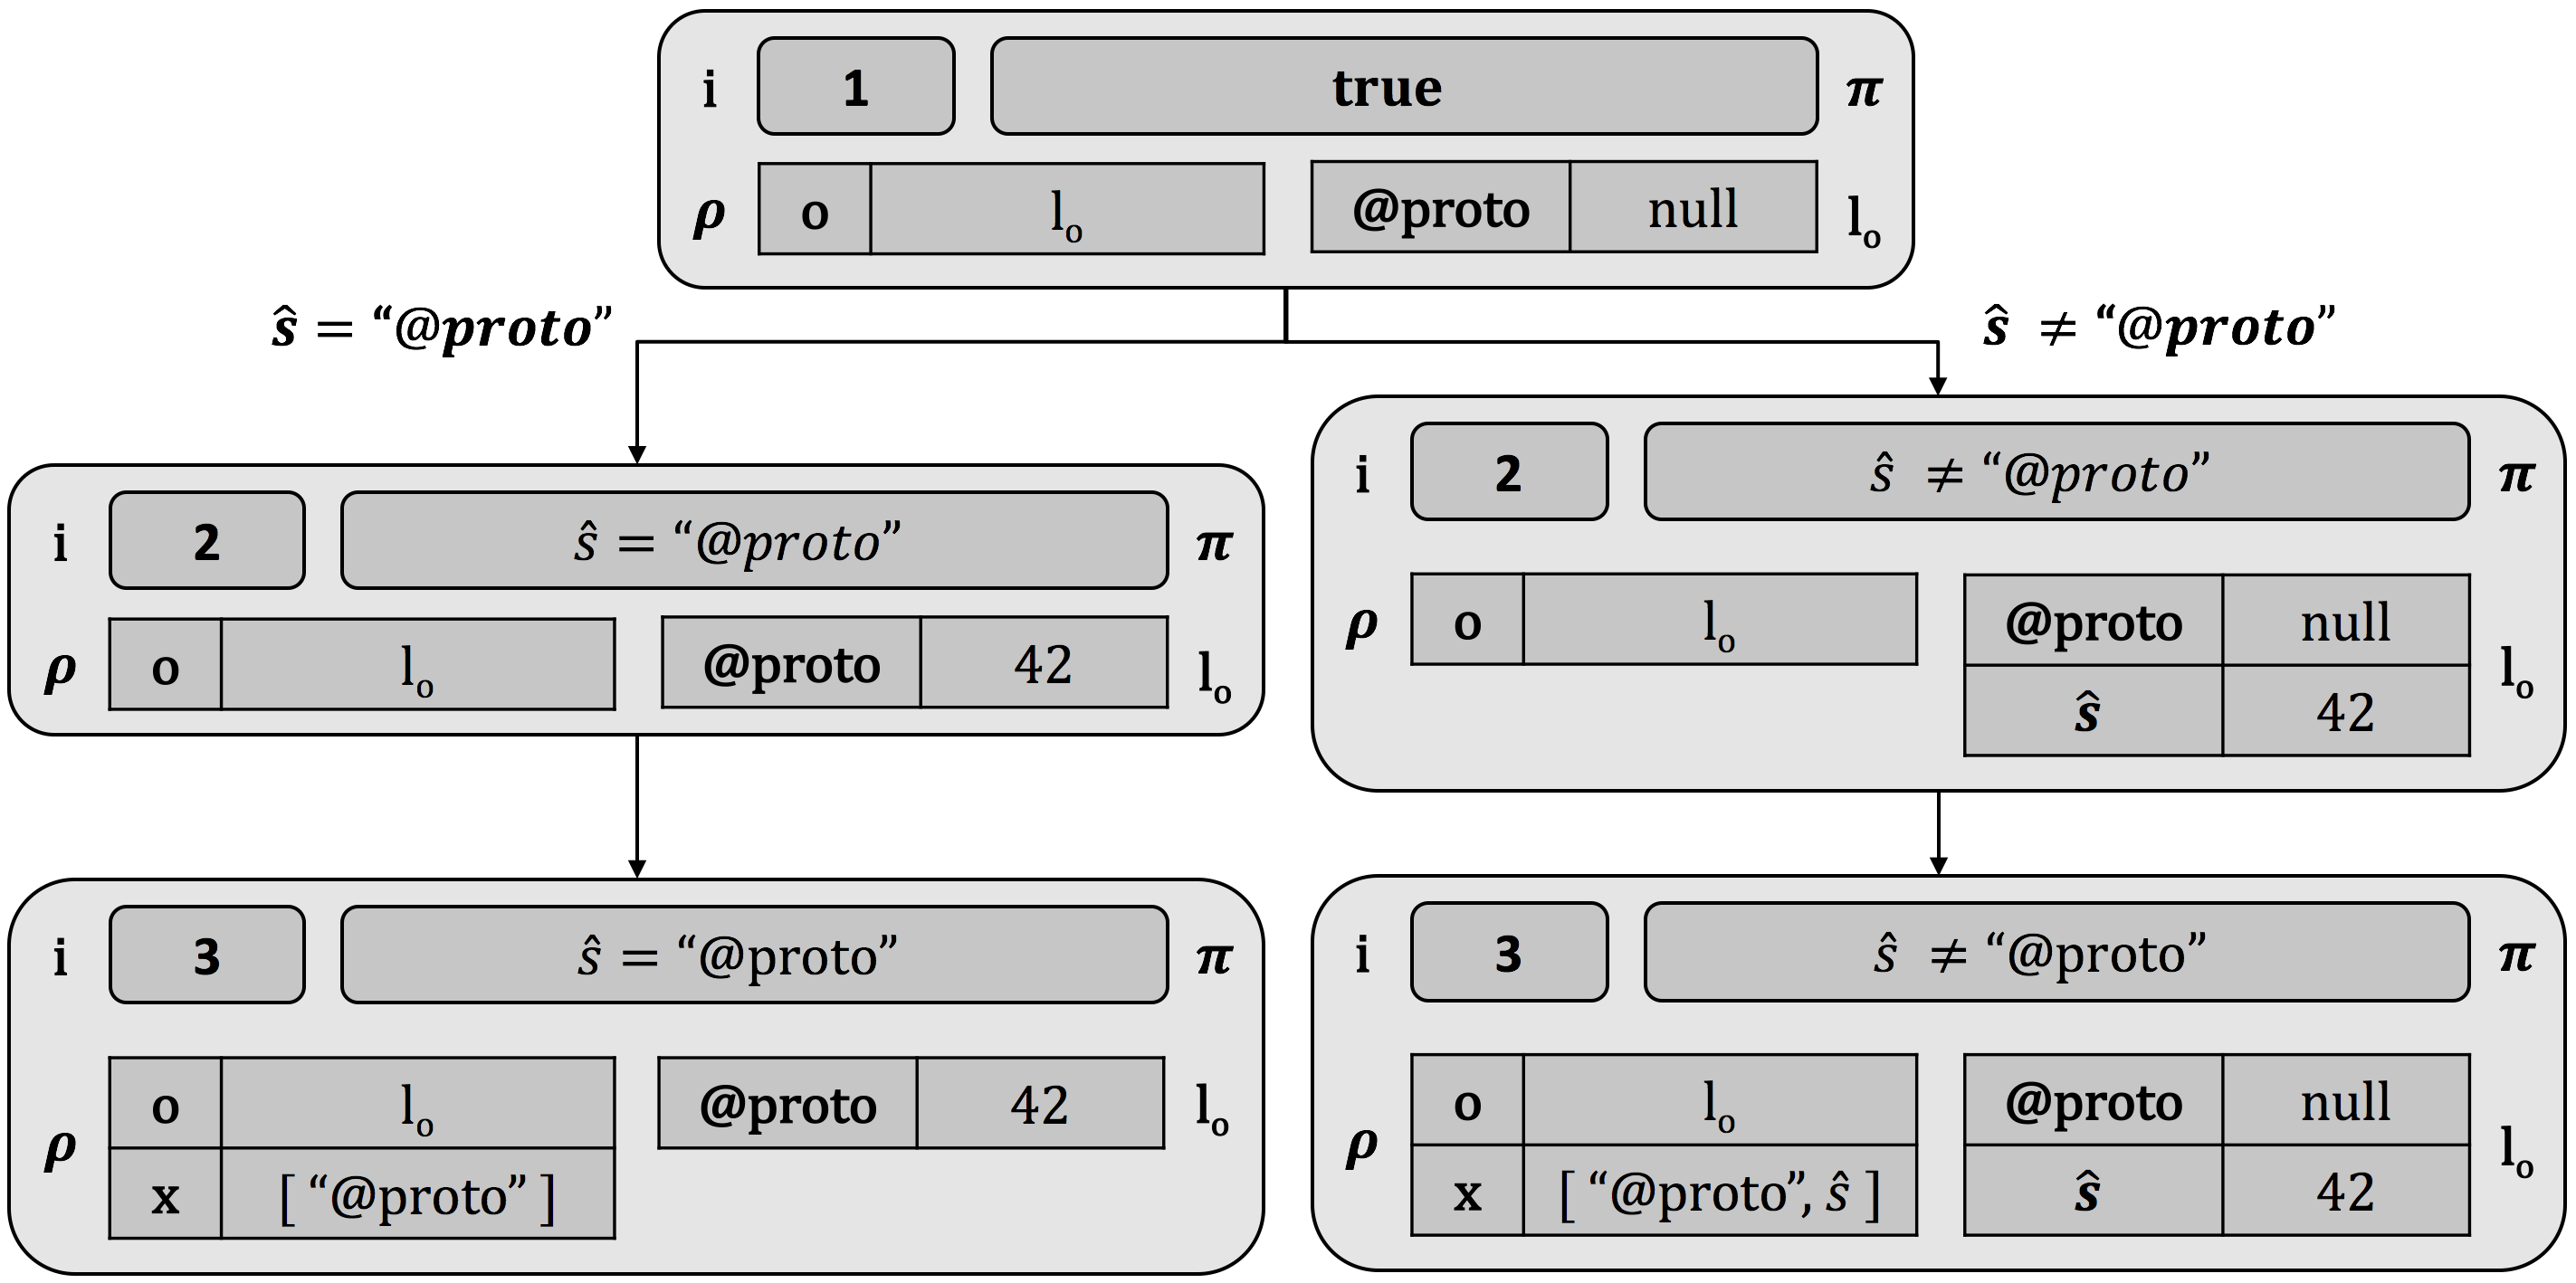
\includegraphics[width=0.83\textwidth]{symbSemEx.png}
\vspace*{-0.1cm}
\caption{Example of a \jilette symbolic execution}
\label{fig:sexecexample}
\vspace*{-0.3cm}
\end{figure}




%\caption{Concrete Semantics Rules}
%\end{figure}


% Given a heap~$\heap$, we denote: a heap cell by $\hcell{\loc}{\jstring}{\val}$, meaning that  $h(\loc,\jstring) = \val$; the union of two disjoint heaps by $\oheap_1 \dunion \oheap_2$; heap lookup by $\hread{\oheap}{\loc}{\jstring}$; and the empty heap by $\hemp$.
%A \jsil variable store, $\store \in \stores$, is a mapping from JSIL program variables $\jvar \in \jvars$ to JSIL values. 



%the heap $\heap'$, store $\store'$, call stack $\ctx'$,   
%and the next command to be evaluated is the $i'$-th command of the first procedure of the call stack~$\ctx'$, in execution mode $\mode'$

%the heap $\heap$, store $\store$, . Due to space constraints and as the transitions for JSIL symbolic execution are  similar, we give the full semantics for JSIL control flow commands in the~Appendix. % So far, so boring.




%We denote the semantic interpretation of unary operators $\unoper$ by $\semop{\unoper}$, the semantic interpretation of binary operators $\binoper$ by $\semop{\binoper}


\subsection{Formal Guarantees}\label{sex:formal:guarantees}

\subsubsection{Preliminaries}
To establish the soundness of symbolic execution, we need to relate 
symbolic states to concrete states. To this end, we make use of \emph{symbolic environments} 
$\senv : \svars \rightharpoonup \vals$, mapping symbolic values to concrete values. 
A symbolic environment is \emph{well-formed} if it maps symbolic 
values to concrete values of the appropriate type (i.e.~symbolic strings are mapped to strings 
and symbolic numbers are mapped to numbers). In the following, we always 
assume well-formed symbolic environments. 
%%
Given a symbolic environment $\senv$, we define the interpretation of symbolic states as follows. 

\begin{display}{Symbolic State Interpretation}
{\scriptsize 
\begin{mathpar}
\inferrule[Symbolic Expressions]
{}{
\interpret{\symbconc}{\senv}(\val) \semeq \val 
%
\qquad
%
\interpret{\symbconc}{\senv}(\svar) \semeq \senv(\svar)
%
\qquad
%
\interpret{\symbconc}{\senv}(\unoper\ \sexpr) \semeq \semop{\unoper} (\interpret{\symbconc}{\senv}(\sexpr))
%
\qquad 
\interpret{\symbconc}{\senv}(\sexpr_1 \binoper \sexpr_2) \semeq \semop{\binoper}(\interpret{\symbconc}{\senv}(\sexpr_1), \interpret{\symbconc}{\senv}(\sexpr_2)) 
}
\\
%
\inferrule[Symbolic Stores]{}{
 \interpret{\symbconc}{\senv}(\storeemp) \semeq \storeemp   
\qquad
\frac{
   \val = \interpret{\symbconc}{\senv}(\sexpr) 
   \quad 
   \store = \interpret{\symbconc}{\senv}(\sstore)
}{
  \interpret{\symbconc}{\senv}((\jvar: \sexpr) \dunion \sstore) \semeq (\jvar: \val) \dunion \store 
}}
\and
\inferrule[Symbolic Contexts]{}{
\interpret{\symbconc}{\senv}(\lstemp) \semeq \lstemp
\qquad
\frac{
    \store = \interpret{\symbconc}{\senv}(\sstore)
    \quad 
    \cs = \interpret{\symbconc}{\senv}(\scs)
}{
\interpret{\symbconc}{\senv}((\pid, \sstore, \jvar, i, j) \lstcons \scs) \semeq (\pid, \store, \jvar, i, j) \lstcons \cs
}}
 \\
 %
\inferrule[Symbolic Heaps]{}{
\interpret{\symbconc}{\senv}(\hemp) \semeq \hemp, \emptyset
\qquad
\frac{
  \begin{array}{c}
   l = \interpret{\symbconc}{\senv}(\sexprl) \quad 
    p =  \interpret{\symbconc}{\senv}(\sexprp) \\
    v =  \interpret{\symbconc}{\senv}(\sexprv) \quad 
    \heap = \hcell{l}{p}{v}
  \end{array}
}{
\interpret{\symbconc}{\senv}(\hcell{\sexprl}{\sexprp}{\sexprv}) \semeq  \heap, \emptyset
}
\qquad
\frac{
  \begin{array}{c}
   l = \interpret{\symbconc}{\senv}(\sexprl) \quad 
   p = \interpret{\symbconc}{\senv}(\sexprp)  \\ 
   \hdom = \jsilset{ (l, p) }
    \end{array}
}{
  \interpret{\symbconc}{\senv}(\hcell{\sexprl}{\sexprp}{\none}) \semeq \hemp, \hdom
}
\qquad
\frac{
  \begin{array}{c}
   \interpret{\symbconc}{\senv}(\sheap_i) = h_i, \hdom_i \mid_{i =1,2} \\ 
   \heap = h_1 \dunion h_2 \quad 
   \hdom = \hdom_1 \dunion \hdom_2
   \end{array}
}{
\interpret{\symbconc}{\senv}(\sheap_1 \dunion \sheap_2) \semeq \heap, \hdom
}}
\\
\inferrule[Symbolic Domains]
{
  \hdom =  \{ (l, p) \mid \sexprl \in \domain(\sdom) \, \wedge \, l = \interpret{\symbconc}{\senv}(\sexprl) 
                 \, \wedge \, p \not\in \interpret{\symbconc}{\senv}(\sdom(\sexprl)) \}
}{
\interpret{\symbconc}{\senv}(\sdom) 
    \semeq \hdom 
}
\and
\inferrule[Symbolic States]{
    \sstate = (\sheap, \sdom, \sstore, \pc) 
    \quad 
   \interpret{\symbconc}{\senv}(\sheap) = \heap, \hdom_1
   \quad
   \interpret{\symbconc}{\senv}(\sdom) = \hdom_2
   \\\\
   \interpret{\symbconc}{\senv}(\sstore) = \store
    \quad 
    \interpret{\symbconc}{\senv}(\pc) = \jtrue 
    \quad 
    \hdom = \domain(h) \cup \hdom_1 \cup \hdom_2 
}{
\interpret{\symbconc}{\senv}(\sstate) \semeq \{ (\heap, \store, \heap_f) \mid \domain(\heap_f) \cap \hdom = \emptyset \} 
}

\end{mathpar}}
\end{display}

\jfs{
\begin{enumerate}
\item Explain the rules. 
\item Explain how the interpretation of symbolic states is not the small footprint interpretation - it takes all the possible compatible frames into account. 
\item Explain how the nones + domains restrict all the possible frames. 
\end{enumerate}
}
 


\subsubsection{Main Results}
The \emph{soundiness theorem} (Theorem~\ref{teo:soundness:jsil:symb:exe}) states that if we have a symbolic trace given by 
$\transabssemrule{\sstate, \scs, i}{\sstate', \scs', j}{\mode}{\mode'}{\symbolic}$ and a concrete CF-state $(\jstate, \cs)$
in the models of the initial symbolic CF-state filtered by the final path condition $\sstate'.\pcsel$,  
then there exists a concrete CF-state $(\jstate', \cs')$ in the models of the final symbolic CF-state, such that: 
$\transabssemrule{\jstate, \cs, i}{\jstate', \cs', j}{\mode}{\mode'}{\concrete}$. 
We use the final path condition $\sstate'.\pcsel$ for both the models of the initial and final 
symbolic states because we only care about the initial concrete CF-states for which 
the concrete execution follows the same path as the symbolic~execution. 

\begin{theorem}[Soundiness]\label{teo:soundness:jsil:symb:exe}
$$
\begin{array}{l}
\transabssemrule{\sstate, \scs, i}{\sstate', \scs', j}{\mode}{\mode'}{\symbolic}  \ \wedge \ (\jstate, \cs, \heap_f) \in \interpret{\symbconc}{\senv}(\sstate \, \wedge \, \sstate'.\pcsel, \scs) \\ \quad \quad 
    \ \implies \ \exists \, \senv', \jstate', \cs' \, . \, 
        \transabssemrule{\jstate \dunion \heap_f, \cs, i}{\jstate' \dunion \heap_f, \cs', j}{\mode}{\mode'}{\concrete}
               \ \wedge \ (\jstate', \cs', \heap_f) \in \interpret{\symbconc}{\senv'}(\sstate', \scs')
\end{array}
$$
\end{theorem}

The \emph{bug-finding} corollary (Corollary~\ref{bug:finding}) states that if 
we find a symbolic trace that results in a failed assertion, 
then there also exists a concrete execution that will cause that assertion to fail.
Observe that the analysis is designed in such a way that there are no false positives, 
meaning that if we find a failing symbolic trace,
we can always instantiate its symbolic values obtaining a concrete counter-model for the 
failing assertion. This is essential, as \jilette is primarily a \emph{bug-finding} tool.


\begin{corollary}[Bug-finding]\label{bug:finding}
$$
\transabssemrule{\sstate, \scs, i}{\sstate', \scs', j}{\mode}{\bot}{\symbolic}  
      \ \implies \  \exists \jstate, \cs \, . \, \transabssemrule{\jstate, \cs, i}{-, -, j}{\mode}{\bot}{\concrete} 
$$
\end{corollary}

Finally, the \emph{verification} corollary (Corollary~\ref{corollary:verification})
states that if we have symbolically explored all the possible execution paths
starting from a given symbolic CF-state $(\sstate, \scs)$,  
then the execution of the program starting from  any concrete state in the models 
of the initial symbolic state (under the initial path condition) will result in a final concrete state
in the models of one of the final symbolic states (under its associated path condition).  
As \jilette does not infer loop invariants, if a \jsil program contains loops that cannot be 
unrolled statically, we will never be in the case of the verification corollary. 

\begin{corollary}[Verification]\label{corollary:verification}
$$
\begin{array}{l}
\wedge_{k=1}^n \, \big( \transabssemrule{\sstate, \scs, i}{\sstate_k, \scs_k, j_k}{\mode}{\mode_k}{\symbolic}  \big)
    \, \wedge \, \big( \sstate.\pcsel \vdash \vee_{k=1}^n \sstate_k.\pcsel \big) 
    \, \wedge \, (\jstate, \cs, \heap_f) \in \interpret{\symbconc}{\senv}(\sstate, \scs)
    \\ \quad \quad
%
      \ \implies \ \exists 1 \leq l \leq n, \senv', \jstate', \cs' \, . \, 
           \transabssemrule{\jstate, \cs, i}{\jstate', \cs', j_l}{\mode}{\mode_l}{\concrete}
           \, \wedge \, 
           (\jstate', \cs', \heap_f) \in \interpret{\symbconc}{\senv'}(\sstate_l, \scs_l)
\end{array}
$$
\end{corollary}

%
The {\bf proofs} of the above results are given in the Appendix. \polish{What do these results mean with respect to related work? How is this maintainable?} 

\subsubsection{Proof Methodology}

\vspace{5pt}
\begin{display}{Instrumented Semantics Rules}
\text{
{\scriptsize
\begin{mathpar} 
 \inferrule[\textsc{GetDomain}]
   { 
        \semexpr{\jsilexpr}{\store} = \loc
      \quad
       \iheap = \iheap' \, \uplus \, \big((\loc, p_i) \mapsto - \big)\mid_{i = 0}^m  
        \\\\
        %
          (\loc,-) \notin \domain (\iheap')  
        \quad
          \jsilset{p_1, ..., p_m} = \idom(\loc)
          \\\\
        \forall_{0 \leq i \leq n} \, \val_i \neq \none 
         \quad 
           \forall_{n < i \leq m} \, \val_i = \none 
   }{  \absgetdomainrule{\instrumented}{(\iheap, \idom, \store), \jsilexpr}{\jsilset{p_1, ..., p_n}}}
  \and
 % 
     \inferrule[\textsc{GetCell - Not Found}]
   { 
         \semexpr{\jsilexpr_1}{\store} = \loc
        \quad 
         \semexpr{\jsilexpr_2}{\store} = p
      \quad
       \iheap = \iheap'' \, \uplus \, \big((\loc, p_i) \mapsto \val_i \big)\mid_{i = 0}^m
      \\\\
       (\loc,-) \notin \domain (\iheap'')
        \quad
        \idom(\loc) = \val_d
        \quad 
       p \not\in \val_d \cup \jsilset{p_i \mid_{i=0}^m})
       \\\\
        \iheap' = \iheap[(\loc, p) \mapsto \none]
       \quad 
       \idom' = \idom[\loc \mapsto \val_d \cup \jsilset{p}]
     }{  \absgetcellrule{\instrumented}{(\iheap, \idom, \store), (\jsilexpr_1, \jsilexpr_2)}{(\iheap', \idom', \store), (\loc, p, \none)}}
  %
  \\
  %
    \inferrule[\textsc{GetCell - Found}]
   { 
         \semexpr{\jsilexpr_1}{\store} = \loc
        \quad 
         \semexpr{\jsilexpr_2}{\store} = p
      \quad
       \iheap = - \, \uplus \, (\loc, p) \mapsto \val
        }{  \absgetcellrule{\instrumented}{(\iheap, \idom, \store), (\jsilexpr_1, \jsilexpr_2)}{(\iheap, \idom, \store), (\loc, p, \val)}}
%
  \and 
   %
    \inferrule[\textsc{Store Update}]
   { 
         \store' = \store[\jvar \mapsto \val]
   }{  \stupdt{\instrumented}((\iheap, \idom, \store), \jvar, \val) =  (\heap, \idom, \store')}
 %
 \and
 % 
       \inferrule[\textsc{Heap Update}]
   { 
         \istate = (\iheap, \idom, \store) 
         \quad 
         \iheap' = \iheap[(\loc, p) \mapsto \val]
   }{  \hpupdt{\instrumented}(\istate, (\loc, p), \val) =  (\iheap, \idom, \store) }
\\
  %
      \inferrule[\textsc{Assume}]
   {}{  \absassume{\instrumented}(\istate, \jtrue) =  \istate }
  \and
    \inferrule[\textsc{Satisfiable}]
   {}{  \abssat{\instrumented}(\istate, \jbool) = \jbool}
     \and
      \inferrule[\textsc{Symbolic Value Creation }]
   {\val \in \vals \text{ is of type } \jtype}{\absmakesymbolicrule{\concrete}{\jtype} = \val}
 \end{mathpar}}}
 \end{display}

\newpage

\begin{display}{Symbolic State Instrumented Interpretation}
{\scriptsize 
\begin{mathpar}
\inferrule[Symbolic Heaps]{}{
\interpret{\symbinst}{\senv}(\hemp) \semeq \hemp
\qquad
\frac{
  \begin{array}{c}
   l = \interpret{\symbconc}{\senv}(\sexprl) \quad 
    p =  \interpret{\symbconc}{\senv}(\sexprp) \\
    v =  \interpret{\symbconc}{\senv}(\sexprv) \quad 
    \heap = \hcell{l}{p}{v}
  \end{array}
}{
\interpret{\symbinst}{\senv}(\hcell{\sexprl}{\sexprp}{\sexprv}) \semeq  \heap
}
\qquad
\frac{
  \begin{array}{c}
   l = \interpret{\symbconc}{\senv}(\sexprl) \quad 
   p = \interpret{\symbconc}{\senv}(\sexprp)  \\ 
      \heap = \hcell{l}{p}{\none}
    \end{array}
}{
  \interpret{\symbinst}{\senv}(\hcell{\sexprl}{\sexprp}{\none}) \semeq \heap
}
\qquad
\frac{
  \begin{array}{c}
   \interpret{\symbconc}{\senv}(\sheap_i) = \iheap_i, \hdom_i \mid_{i =1,2} \\ 
   \iheap = \iheap_1 \dunion \iheap_2 
   \end{array}
}{
\interpret{\symbinst}{\senv}(\sheap_1 \dunion \sheap_2) \semeq \iheap
}}
\\
\inferrule[Symbolic Domains]
{
   \idom(\loc) = \val  \iff  \exists \sexprl \in \domain(\sdom) \, . \,  \loc = \semexpr{\sexprl}{\senv} \, \wedge \, \val = \semexpr{\sdom(\sexprl)}{\senv}
}{
\interpret{\symbinst}{\senv}(\sdom) \semeq \idom
}
\and
\inferrule[Symbolic States]{
    \sstate = (\sheap, \sdom, \sstore, \pc) 
    \quad 
    \interpret{\symbinst}{\senv}(\sheap) = \iheap
   \quad
    \interpret{\symbinst}{\senv}(\sdom) = \idom
    \\\\
    \interpret{\symbconc}{\senv}(\sstore) = \store 
    \quad
    \interpret{\symbconc}{\senv}(\pc) = \jtrue 
}{
\interpret{\symbinst}{\senv}(\sstate) \semeq (\iheap, \idom, \store)
}
\end{mathpar}}
\end{display}

\begin{theorem}[Soundiness wrt Instrumented Semantics]\label{lemma:soundness:jsil:symb:exe:instrumented:instrumented}
$$
\begin{array}{l}
\transabssemrule{\sstate, \scs, i}{\sstate', \scs', j}{\mode}{\mode'}{\symbolic}  \ \wedge \ (\istate, \cs) = \interpret{\symbinst}{\senv}(\sstate \, \wedge \, \sstate'.\pcsel, \scs) \\ \quad \quad 
    \ \implies \ \exists \, \senv', \istate', \cs' \, . \, 
        \transabssemrule{\istate, \cs, i}{\istate', \cs', j}{\mode}{\mode'}{\instrumented} \ \wedge \ (\istate', \cs') = \interpret{\symbinst}{\senv'}(\sstate', \scs')
\end{array}
$$
\end{theorem}


\begin{display}{Instrumented State Interpretation}
{\scriptsize 
\begin{mathpar}
\inferrule[Symbolic Heaps]{}{
\interpret{\instconc}{}(\hemp) \semeq \hemp
\quad
\frac{
   \heap = \hcell{\loc}{p}{\val}
}{
\interpret{\instconc}{}(\hcell{\loc}{p}{\val}) \semeq  \heap
}
\quad
  \interpret{\instconc}{}(\hcell{\loc}{p}{\none}) \semeq \hemp }
\quad
\frac{
  \begin{array}{c}
   \interpret{\instconc}{}(\iheap_i) = \heap_i, \hdom_i \mid_{i =1,2} \\
   \heap = \heap_1 \dunion \heap_2
  \end{array}
}{
\interpret{\instconc}{}(\iheap_1 \dunion \iheap_2) \semeq  \heap
}
\qquad
\inferrule[Symbolic States]{
    \interpret{\instconc}{}(\iheap) = \heap
}{
\interpret{\instconc}{}(\iheap, \idom, \store) \semeq (\heap, \store)
}
\end{mathpar}}
\end{display}

\begin{theorem}[Frame Property - Instrumented Semantics]\label{teo:frame:property}
$$
\begin{array}{l}
\transabssemrule{\istate, \cs, i}{\istate', \cs', j}{\mode}{\mode'}{\instrumented} 
       \ \implies \ 
        \transabssemrule{\istate \dunion \iheap_f, \cs, i}{\istate' \dunion \iheap_f, \cs', j}{\mode}{\mode'}{\instrumented} 
\end{array}
$$
\end{theorem}

\begin{lemma}[Instrumented Semantics Interpreation]\label{lemma:instrumented:semantics}
$$
\begin{array}{l}
\transabssemrule{\istate, \cs, i}{\istate', \cs', j}{\mode}{\mode'}{\instrumented} 
   \, \wedge \, \interpret{\instconc}{}(\istate) =  \jstate
      \, \wedge \, \interpret{\instconc}{}(\istate') =  \jstate'
       \ \implies \ 
        \transabssemrule{\jstate, \cs, i}{\jstate', \cs', j}{\mode}{\mode'}{\concrete} 
\end{array}
$$
\end{lemma}



\begin{lemma}[Two-Level Symbolic Interpretation]\label{lemma:symb:interpretation}
$$
(\jstate, \cs, \heap_f) \in \interpret{\symbconc}{\senv}(\sstate, \scs) 
   \iff 
   \exists \, \istate, h_F \, . \, 
         (\istate, \cs) = \interpret{\symbinst}{\senv}(\sstate, \scs)  
          \ \wedge \   
      \jstate = \interpret{\instconc}{}(\istate)
      \ \wedge \
      h_F \disjoint \istate.\hpsel
$$
\end{lemma}

\myparagraph{Soundiness - Proof} 
We show how the intermediate results can be used together to 
obtain the soundiness theorem (Theorem~\ref{teo:soundness:jsil:symb:exe}). 
Assume we have that 
$\transabssemrule{\sstate, \scs, i}{\sstate', \scs', j}{\mode}{\mode'}{\symbolic}$ (\hyp{1}) and 
 $(\jstate, \cs, \heap_f) \in \interpret{\symbconc}{\senv}(\sstate \, \wedge \, \sstate'.\pcsel, \scs)$ (\hyp{2}).  
 From \hyp{2}, we conclude, using Lemma~\ref{lemma:symb:interpretation}, that there is an 
 instrumented state $\istate$ and a heap $\heap_f$ such that $(\istate, \cs) = \interpret{\symbinst}{\senv}(\sstate  \, \wedge \, \sstate'.\pcsel, \scs)$ (\ieq{1}), 
 $\jstate = \interpret{\instconc}{}(\istate)$ (\ieq{2}), and $h_F \disjoint \istate.\hpsel$ (\ieq{3}). 
 Applying Theorem~\ref{lemma:soundness:jsil:symb:exe:instrumented:instrumented} to \hyp{1} 
 and \ieq{1}, it follows that there is a symbolic environment $\senv'$, an instrumented state $\istate'$, 
 an a call stack $\cs'$ such that: 
$\transabssemrule{\istate, \cs, i}{\istate', \cs', j}{\mode}{\mode'}{\instrumented}$~(\ieq{4})
and $(\istate', \cs') = \interpret{\symbinst}{\senv'}(\sstate', \scs')$ (\ieq{5}).
From \ieq{3} and \ieq{4}, we conclude, using Theorem~\ref{teo:frame:property}, that the following 
holds $\transabssemrule{\istate \dunion \heap_f, \cs, i}{\istate' \dunion \heap_f, \cs', j}{\mode}{\mode'}{\instrumented}$ (\ieq{6}). 
Applying Lemma~\ref{lemma:instrumented:semantics} to \ieq{2} and \ieq{6}, we conclude that 
 $\transabssemrule{\jstate \dunion \heap_f, \cs, i}{\jstate' \dunion \heap_f, \cs', j}{\mode}{\mode'}{\instrumented}$ (\goal{1}), 
 where $\jstate' = \interpret{\instconc}{}(\istate')$ (\ieq{8}).
 From \ieq{5}, \ieq{6}, and \ieq{8}, we conclude, applying Lemma~\ref{lemma:symb:interpretation}, 
 that $(\jstate', \cs', \heap_f) \in \interpret{\symbconc}{\senv}(\sstate', \scs')$ (\goal{2}), 
 which concludes the proof. 

\subsection{Implementation}\label{subsec:jsil:analysis:implementation}


Implementing a symbolic execution engine for \jsil is a non-trivial 
task, requiring a substantial engineering effort. 
% 
% 
Hence, instead of implementing the symbolic semantics of \jsil from scratch, we leverage on 
\rosette~\cite{Rosette1,Rosette2}, a symbolic virtual machine designed to 
enable swift development of new 
solver-aided languages. 
%
\rosette is a small extension of Racket~\cite{racket} equipped with a symbolic compiler with support 
for symbolic values and first order assertions. Because \rosette is itself solver-aided, languages 
implemented in \rosette can also make use of the solver-aided facilities provided by \rosette. 
Hence, by implementing a \emph{concrete} \jsil interpreter in \rosette, we obtain \emph{for free} a symbolic 
interpreter for \jsil. %consistent with the symbolic semantics described in  \S\ref{subsec:jsil:analysis:formalism}. 
%The idea of turning a concrete interpreter into a symbolic interpreter by embedding it in 
%
The implementation of the concrete interpreter in \rosette must fulfil the following criteria:

\begin{itemize}          
   \item \emph{Efficiency:} the implementation must promote \rosette's efficient behaviour;
   
   \item \emph{Termination:} the user must be given a way to establish a bound for the symbolic execution 
            of programs that loop on symbolic values; 
  
   \item \emph{Adequacy:} the symbolic execution of the concrete interpreter in \rosette 
            must be consistent with the symbolic semantics described in \S\ref{subsec:jsil:analysis:formalism}. 
\end{itemize}

\subsubsection{Efficiency}
It is often possible for more than one transition of the symbolic 
semantics to be applicable during symbolic execution, 
giving rise to a potentially intractable number of possible symbolic states. 
To counter this problem, \rosette uses a sophisticated 
symbolic state merging algorithm, which factors out the common 
part between multiple symbolic states  in order to expose more 
opportunities for concrete evaluation. The non-mergeable portions of the state 
are represented as \emph{guarded symbolic unions}. 
Our goal is to write the interpreter code in a way that helps 
\rosette merge sets of possible symbolic states, yielding minimal 
guarded symbolic unions.

\subsubsection{Termination} The \jsil symbolic execution engine does not 
include the abstraction mechanisms which would allow it to finitise the symbolic 
execution of loops depending on symbolic values~\cite{abstract:symbolic:exec}. 
Hence, the user is asked to specify an upper bound on the number of times
the symbolic execution is allowed to branch on symbolic values by using
conditional gotos. 
Once that upper bound is reached, if a conditional goto that branches 
on a symbolic value is encountered, the symbolic execution stops.  




